\documentclass[pdflatex,a4paper]{article}

\usepackage{pgffor, ifthen}
\newcommand{\notes}[3][\empty]{%
    \noindent \vspace{10pt}\\
    \foreach \n in {1,...,#2}{%
        \ifthenelse{\equal{#1}{\empty}}
            {\rule{#3}{0.5pt}\\}
            {\rule{#3}{0.5pt}\vspace{#1}\\}
        }
}

\usepackage{graphicx}

\usepackage[margin=3cm]{geometry}

\title{Practical 12. Modelling infections}

\author{MI Stefan}

\date{IBI1, 2018/19}


\usepackage{url}
\usepackage{amsmath}

\usepackage{listings}
\lstset{language=python}


\begin{document}

\newcommand{\<}{\textless}
\renewcommand{\>}{\textgreater}


\maketitle

\section{Learning objectives}


\begin{itemize}
\item
Encode real-world problems as probabilistic models	
\item
Implement a stochastic SIR (Susceptible-Infected-Recovered) model in Python
\end{itemize}

\section{Introduction}

SIR models (\textbf{S}usceptible - \textbf{I}nfected - \textbf{R}ecovered or \textbf{R}esistant) are used to study how infectious diseases spread through a population. In its simplest form, the model assumes that the population being studied falls into three separate groups: Susceptible individuals (S) are healthy, but may contract the disease. Infected people (I) have contracted the disease and can pass it on to susceptible people at a rate that depends on an infection probability upon contact \(\beta\) (beta) and on the proportion of infected people in the population. An infected person can recover (R) with recovery probability \(\gamma\) (gamma), and is assumed to be immune to the disease after recovery.  

Though simple, SIR models can be very informative. They can be extended and modified in many ways to account for specific diseases, interventions, incubation periods, or other factors. 

SIR models can be deterministic or probabilistic - in this practical, we will look at four different probabilistic models. We will build the models step-by-step, using tools you have encountered before or that are supplied in this practical guide. As often in programming, there are more than one correct ways to do something, so if you have a good idea, feel free to use it!


\section{A simple SIR model}

\begin{itemize}
\item
Make a new python script called \verb=SIR.py=
\item
At the beginning, you have to import the relevant python libraries in order to have access to some of the functions we need. Start with that.

\begin{lstlisting}
# import necessary libraries
import numpy as np
import matplotlib.pyplot as plt
\end{lstlisting}

\item

Next, define the basic variables of the model, one for each of the population (Susceptible, Infected, and Recovered). Initially, we start with a population of 10\,000 people. Initially, one person is infected, the rest of the population is Susceptible (nobody has yet recovered). It also makes sense to define a variable N that holds the total number of people in the population. You also want to define beta and gamma. Here, we use 0.3 for beta and 0.05 for gamma. 

\item

You will also want to create arrays for each of your variables to track how they evolve over time. (Recall that you can define an array using square brackets \verb=[]= and that you can later add elements to an array using the \verb=append()= function). 

\item
Now comes the heart of this problem: The time course. We will loop over 1000 time points. At each time point, we pick susceptible individuals at random to become infected. We pick infected individuals at random to become recovered. And we then keep track of the numbers of people in all three categories. 
\begin{itemize}
\item
Before you get into the coding of the time loop, write out what you will need in pseudocode
\item
You may find the \verb=random.choice= function helpful, which is provided by \verb=numpy=. Random choice takes three arguments: First the set from which to choose elements, second the number of elements to be chosen and third a list of probabilities for choosing each member of a set. For instance, the command \verb*np.random.choice(range(2),4,p=[0.8,0.2])* will choose numbers from \verb=range(2)= (i.e. \(0\) or \(1\)) four times, with a probability of \(0.8\) of choosing \(0\) and a probability of \(0.2\) of choosing \(1\). In other words, it will give you a list of ones and zeros of length four, of which there are approximately \(80\,\%\) zeroes. 
\item
A note on probabilities: The recovery probability for each infected individual is easy: it is just gamma. The probability of infection is a bit trickier. For a susceptible individual to be infected, you have to consider not only the infection rate upon contact (beta), but also the probability of making contact with an infected individual. We account for this by multiplying beta by the proportion of infected people in the population.
\item
Before moving on to the next time step, make sure you record the output of each time step (i.e. the number of susceptible, infected, and recovered individuals) 
\end{itemize}

\item
  Finally, you want to plot your results: Plot the numbers of susceptible, infected, and recovered people as a function of time. You have used \verb=matplotlib.pyplot= before. The functions you may be especially interested in include \verb=plot()=, \verb=xlabel()=, \verb=ylabel(1)=, \verb=title()=, \verb=legend()=

Our own figure looked something like this:

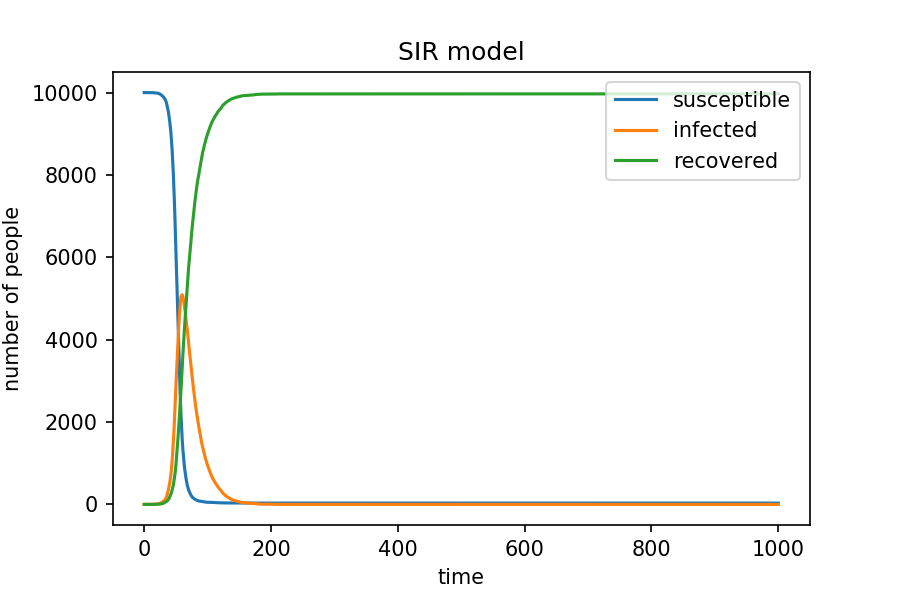
\includegraphics{SIR.png}

\item
Here is a useful trick if you want to save your plots as a file. Before starting the plot, set up its dimensions and resolution:

\begin{lstlisting}
plt.figure(figsize=(6,4),dpi=150)  
\end{lstlisting}

Then when you are done specifying your plot, you can save it as

\begin{lstlisting}
plt.savefig("<filename>",type="png")    
\end{lstlisting}

Note that Python is not necessarily saving images in the same directory that your python scripts are in. You can get around it by specifying the full file path as \verb=<filename>=.

\item
Now, look at your model. Are you surprised by the outcome? How do you know it works? What happens if you run it several times? What does it look like if you run it with a (much) smaller population? What if you change beta and gamma?
\end{itemize}

\section{The effect of vaccination}

Maybe you have heard about ``herd immunity'', the idea that a population will be immune to a disease if ``enough'' people are vaccinated against it. (This is because vaccinated people cannot be infected and will therefore slow the spread of disease). Importantly ``enough'' does not necessarily mean everybody. Different diseases have different ``herd immunity thresholds'' - this is the percentage of people that need to be vaccinated to prevent the disease from spreading. 

\begin{itemize}
\item
Copy your file \verb=SIR.png= to a new file \verb=SIR_vaccination.py= (It is usually not good practice to code, but for today it's fine).
\item
Can you extend your model to include an additional group of vaccinated people? Can you make it to be \(10\,\%\) of the population? Can you even try different percentages and plot the number of infected people for each of them? 

Here is what it looked like when we did it (but yours may be a bit different, it is a stochastic model after all)

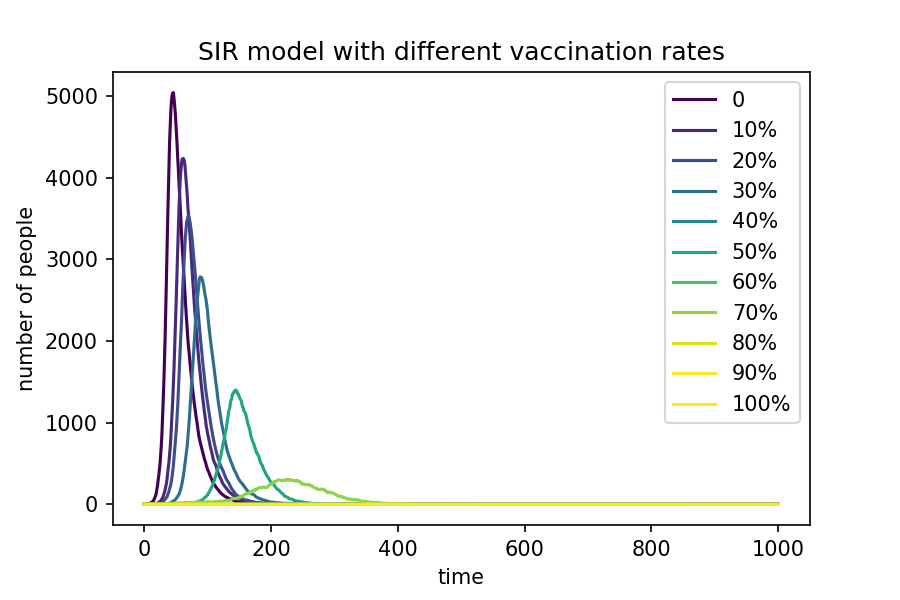
\includegraphics{SIR_vaccine.png}

\item

From looking at your plot, what do you think the herd immunity threshold may be (approximately) for this particular disease?

\newpage

\item
\textbf{Optional:} Interested in using the same nice colour scheme? This can be done using \verb=cm= (for colour map). Import it at the beginning of your document

\begin{lstlisting}
from matplotlib import cm
\end{lstlisting}

Then you can use one of matplotlib's internal colour maps in your plots. For instance:

\begin{lstlisting}
plt.plot(data,color=cm.viridis(30))
\end{lstlisting}

plots the dataset \verb=data= using colour number 30 (a sort of blue) from the viridis colour map. 

You can read more about colour maps in python here: \url{https://matplotlib.org/tutorials/colors/colormaps.html}

\end{itemize}

\section{Looking at disease spread in 2D}

THe SIR model you made assumed that you have essentially a ``well-mixed'' population: A susceptible person on the South side of town is as likely to run into an infected person on the North side as they are to run into their neighbour. This is a simplification that is sometimes ok, but sometimes we want to account for spatial effects.

In this part of the practical, we will make a 2D SIR model. This could, for instance, be used to model the spread of a disease in a given geographical area. This is a bit more difficult, so we will provide some snippets of code here for you to use. (Though please feel free to use your own solution if you have one that works!)

\begin{itemize}
\item
Make file \verb=spatial_SIR.py=
\item
Again, start by importing useful libraries:
\begin{lstlisting}
# import necessary libraries
import numpy as np
import matplotlib.pyplot as plt
\end{lstlisting}
\item
This time, we encode the different states not in the form of variables, but in the form of numbers in an array: \(0\) for susceptible, \(1\) for infected, \(2\) for recovered. We begin by making a \(100\times 100\) array that is completely made of zeroes:

\begin{lstlisting}
# make array of all susceptible population
population = np.zeros( (100, 100) )
\end{lstlisting}

This creates an ``array of arrays'': There are 100 rows and 100 columns, all of which are zero. If you want to look at or change the content of a specific row or column, you use square brackets that contain the row number and the column number, separated by a comma. For instance, if you want to check what number is in row 4, column 12, the command would be

\begin{lstlisting}
population[4,12]
\end{lstlisting}


\item
Again, we will start with exactly one infected person. But this time, we will choose one random point in our \(100\times 100\) array for where the outbreak happens. \emph{How would you do that?}

\newpage

Exactly! \verb-np.random.choice()- The only part about this that is a bit finicky is that this function returns an array, so we have to call on the elements of that array separately. The order of events is this: First we randomly select the x and y coordinates of where the outbreak is happening and store this in an array called outbreak. Then we use this to address the person with those exact coordinates in our population array and change their status from 0 (susceptible) to 1 (infected).


\begin{lstlisting}
outbreak = np.random.choice(range(100),2)
population[outbreak[0],outbreak[1]] = 1
\end{lstlisting}

\item
Let's plot this, and to do this, we use a kind of heat map, where we colour each of the \(10\,000\) points on our map by state (susceptible or infected).  

\begin{lstlisting}
plt.figure(figsize=(6,4),dpi=150)   
plt.imshow(population, cmap='viridis', interpolation='nearest')
\end{lstlisting}

What you should see is a big purple square (all susceptible people) with only one small dot at a random position representing the one infected person (in yellow):

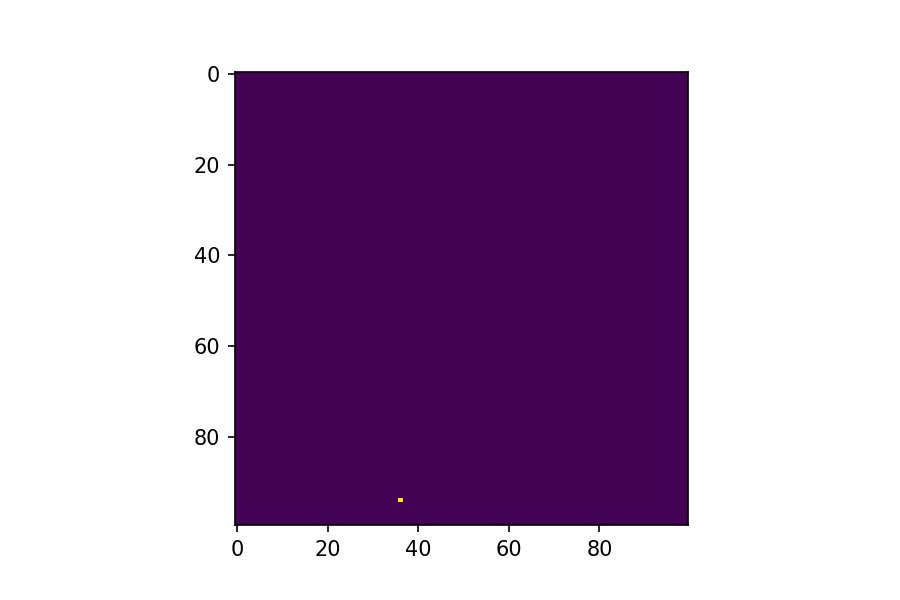
\includegraphics{spatial_SIR0.png}

\item

Before we start setting up the time course simulation, again set up your model parameters, beta and gamma, like you did before. Easy!

\item

For this exercise, we will loop just through 100 time points. At each time point, an infected individual can infect any of its 8 neighbours with infection probability beta. (This is now independent of the number of infected individuals, because we are looking at direct neighbour-to-neighbour infection). Also, an infected individual can recover at rate gamma.

What you want is a heat map for each time point, so that at the end, you can follow the progression of disease through space and time. For instance, here is our model at times 0, 10, 50, and 100. On this heat map, susceptible individuals are shown in dark purple, infected individuals in blue-green and recovered individuals in yellow.
 
\begin{minipage}{\textwidth}
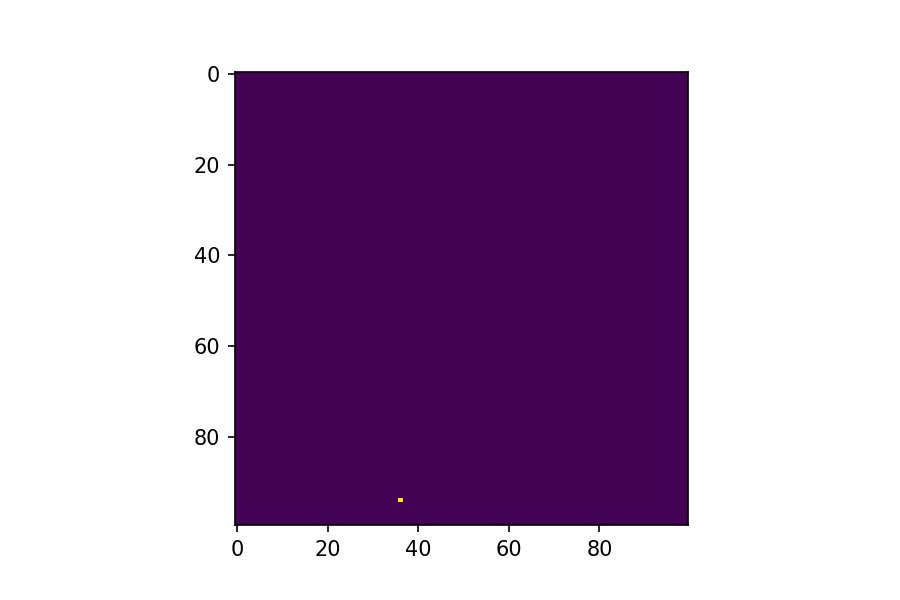
\includegraphics[width=0.5\textwidth]{spatial_SIR0.png}
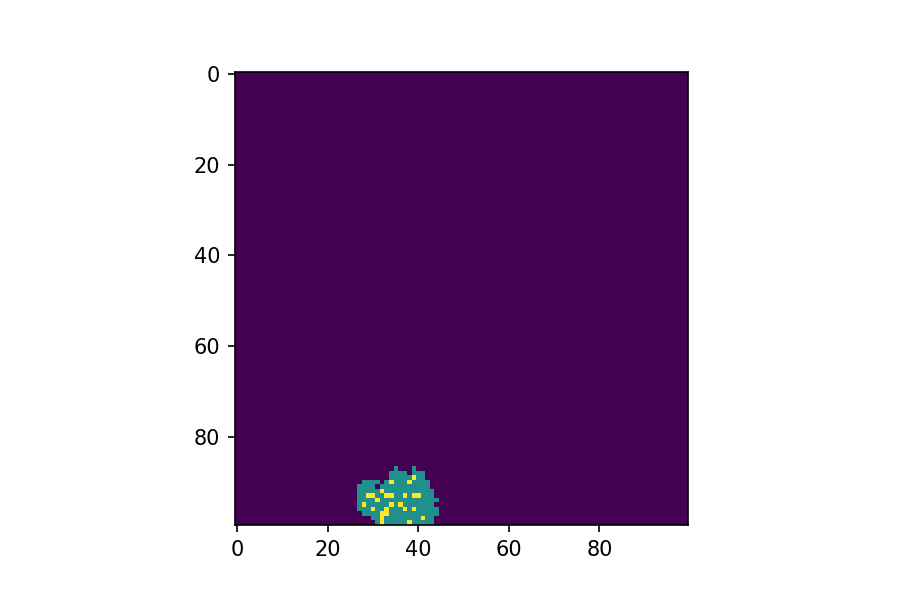
\includegraphics[width=0.5\textwidth]{spatial_SIR10.png} \\
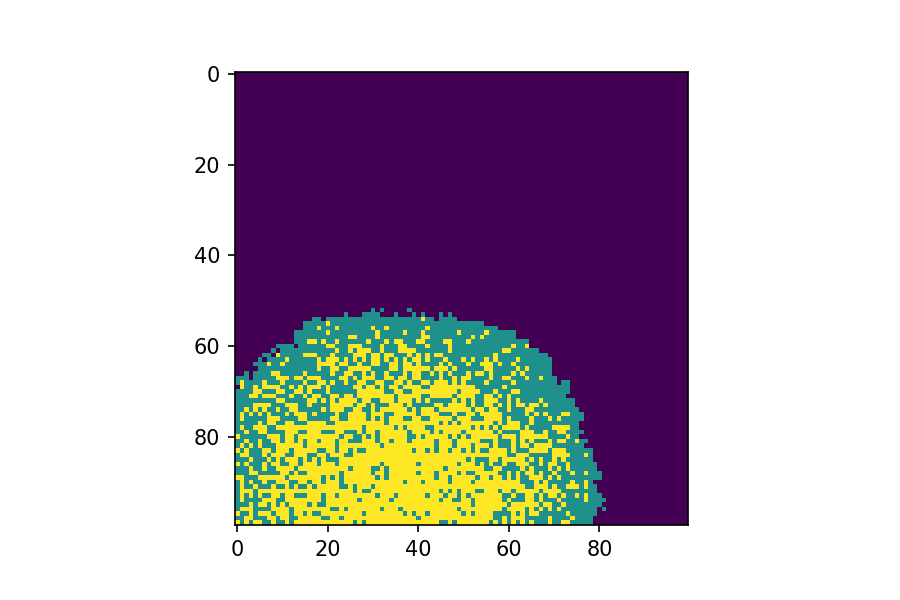
\includegraphics[width=0.5\textwidth]{spatial_SIR50.png}
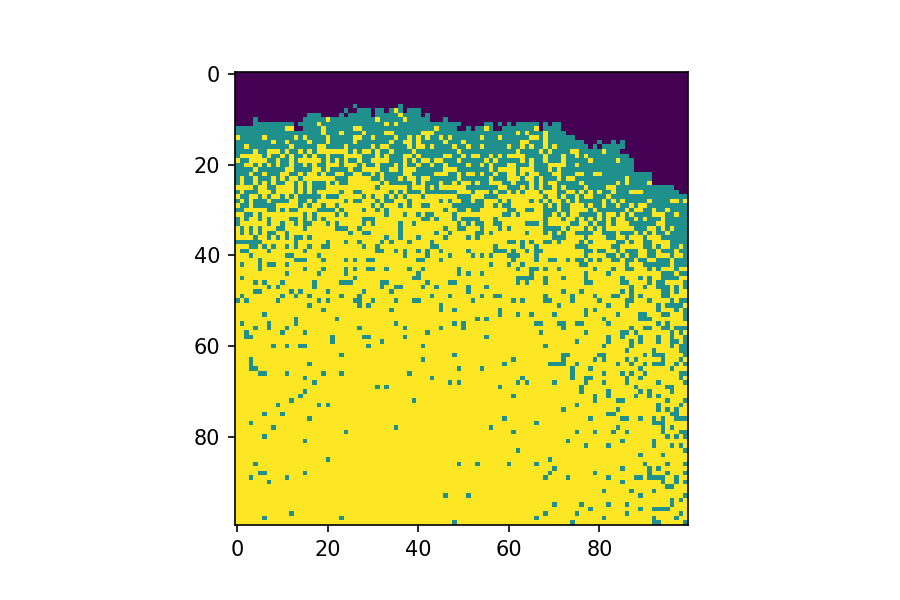
\includegraphics[width=0.5\textwidth]{spatial_SIR100.png}
\end{minipage}




Think through what you need to do at each time point to make this happen and plan it using pseudocode. Here are some things to think about \emph{before you start coding!}:

\begin{itemize}
\item
How will you find the infected points? There are several ways to do this, but you may be interested in the \verb=where()= function that \verb=numpy= provides.
\item
For each infected point, how do you address all its neighbours? Are there cases where this could be difficult?
\item
How do you check that neighbours are not recovered?
\item
How do you infect the neighbours?
\item
How do you allow infected individuals to recover?
\item
How can you plot the outcome? (You don't need to worry about saving the images for now, unless you want to)
\end{itemize}


\item
Ready to actually code? \textbf{You can get help!} You are welcome to implement the entire exercise yourself. But if you feel like you are struggling, or you are short of time (or if you just want to see what it looks like when it works), you can copy and paste the code snippet in the practical folder: \verb=infection_snippet.py= This will take care of finding points that are infected and infecting its neighbours. It \emph{does not} take care of recovery, or of plotting the outcomes - that is your job! 

\item
\textbf{Extra bonus exercise:} What about a spatial SIR model that includes a certain proportion of the population being vaccinated? How would you do that? (Not assessed!) 

\end{itemize}





\section{For your portfolio}

The markers will look for and assess the following:

\begin{description}
\item[File SIR.py] $\;$\\

\begin{itemize}
\item
File exists
\item
Population size, beta, and gamma are defined as specified in the exercise 
\item
The code can be run to produce a plot like the one shown in the exercise. Axes and curves need to be correctly labelled.
\item
Running the code several times produces different results, evidencing that this is a probabilistic model 
\end{itemize}

\item[File SIR\_vaccination.py]$\;$\\

\begin{itemize}
\item
File exists
\item 
A fraction of the population can be vaccinated, but the overall number of individuals is still 10000.
\item
The code produces a figure similar to that shown, with ``infected'' curves for 0, 10, 20, \dots 100 percent vaccination. Axes and curves are correctly labelled
\item
Running the code several times produces different results, evidencing that this is a probabilistic model
\end{itemize}
\item[File spatial\_SIR.py]$\;$\\

\begin{itemize}
\item
File exists
\item
The random selection of one infected individual and plotting of this works
\item
The procedures used are well documented using pseudocode
\item
There is an attempt at propagating infection from infected cells to its neighbours (though there may be minor errors). Using the provided code snippet is fine, as long as it is used correctly
\item
Infected cells can recover, as specified
\item
The code produces a series of plots that show the propagation first of the disease, then of resistance against it. (These can be console plots, no need to produce png images.
\item
Running the code several times produces different results, evidencing that this is a probabilistic model
\end{itemize}

\item[File Reflection.txt]$\;$\\

\begin{itemize}
\item
File exists
\item
File contains reflections on how the practical went. For instance: Was it easy? Was it hard? Were there bits you enjoyed more (or less) than others? What was the most important thing you learned? 
\end{itemize}

\end{description}



You can add or edit things after the Practical session. We do not look at the commit date, we just want it all to be there!

\end{document}


